\newcommand{\lv}[1]{#1}
\newcommand{\sv}[1]{}
\newcommand{\lsv}[2]{\lv{#1}\sv{#2}}
\documentclass{llncs}

\usepackage{times}



\usepackage{tikz}
\usetikzlibrary{positioning,calc}

\usepackage{url}
\usepackage{amsmath,amssymb}
\usepackage{xspace,tikz,enumitem}
\usepackage{mathrsfs,verbatim}
\usepackage{enumitem,todonotes,microtype}

\usepackage{color}
\usepackage{boxedminipage}

\newcommand{\red}[1]{{\color[rgb]{.5,0,0}{#1}}}

\usepackage[]{algorithm2e}





\newcommand{\Nat}{\mathbb{N}}
\newcommand{\hy}{\hbox{-}\nobreak\hskip0pt}

\newcommand{\lab}{\ell} 
\newcommand{\bigoh}{\mathcal{O}}

\def\hy{\hbox{-}\nobreak\hskip0pt} 

\newcommand{\SB}{\{\,} \newcommand{\SM}{\;{|}\;} \newcommand{\SE}{\,\}}
\newcommand{\SBb}{\big\{\,} \newcommand{\SEb}{\,\big\}}
\newcommand{\Card}[1]{|#1|}
\newcommand{\CCard}[1]{\|#1\|}

\newcommand{\BB}{\mathcal{B}} 
\newcommand{\CC}{\mathcal{C}} 
\newcommand{\DD}{\mathcal{D}} 
\newcommand{\FF}{\mathcal{F}} 
\newcommand{\WW}{\mathcal{W}} 
\newcommand{\RR}{\mathcal{R}} 

\newcommand{\NP}{\text{\normalfont NP}}
\newcommand{\coNP}{\text{\normalfont co-NP}}
\newcommand{\FPT}{\text{\normalfont FPT}}
\newcommand{\XP}{\text{\normalfont XP}}
\newcommand{\PSPACE}{\text{\normalfont PSPACE}}
\newcommand{\SPACE}{\text{\normalfont SPACE}}
\newcommand{\TIME}{\text{\normalfont TIME}}
\newcommand{\W}[1][xxxx]{\text{\normalfont W}[#1]}
\newcommand{\coW}[1][xxxx]{\text{\normalfont co-W}[#1]}

\newcommand{\mtext}[1]{\text{\normalfont\itshape #1}} 


\def\caneqf#1#2#3{\approx_{#1,#3}^{\,#2}}
\def\caneq#1#2{\approx_{#1,#2}}
\def\oplus{\mathop{\mbox{}}}


\newcommand{\gleq}{\mathop{\diamondsuit}}




\newcommand{\nb}[1]{\todo{\scriptsize #1}}
\def\pplus#1#2{\,\pplusox{#1\,|\>#2}\,}
\def\pplusox#1{\mathop{\mbox{}}}
\def\pplusoid{\mathop{\mbox{}}}
\def\mx#1{\mbox{\boldmath}}
\def\prebox#1{\mathop{\mbox{\sl#1}}}
\def\MS#1{\mbox{MSO}}

\newcommand{\MSO}{\mbox{MSO}\xspace}

\def\lMS{\mbox{\textsc{LinEMS}}}
\def\lMSp{\mbox{\textsc{LinEMS}}(\phi,d)}
\def\rlMS#1{\mbox{LinEMS}_{#1}}
\def\TT{{\mathcal T}}
\def\AA{{\mathcal A}}
\def\DD{{\mathcal D}}
\def\YY{{\mathcal Y}}
\def\UU{{\mathcal U}}
\def\HH{{\mathcal H}}
\def\MM{{\mathcal M}}
\def\PP{{\mathcal P}}
 



\spnewtheorem{ourfact}{Fact}{\bfseries}{\itshape}
\spnewtheorem{observation}{Observation}{\bfseries}{\itshape}






\def\sm{split-module}
\def\smpar{split partition}
\def\GLT{graph-labeled tree}
\def\wsm{well-structured modulator}
\def\ws{well-structured}

\newcommand{\MSOMC}[1]{\textsc{MSO-MC}}
\newcommand{\MSOOPT}[2]{\textsc{MSO-Opt}}
\newcommand{\MSOCOU}[2]{\textsc{MSO-Count}}

\newcommand{\wsn}{\text{\normalfont\slshape wsn}}
\newcommand{\rw}{\text{\normalfont\slshape rw}}
\newcommand{\md}{\text{\normalfont\slshape mod}}


\pagestyle{plain}

\begin{document}



\title{Solving Problems on Graphs of High Rank-Width\thanks{Supported by the Austrian Science Fund (FWF), project P26696.}}

\author{Eduard Eiben \and Robert Ganian \and Stefan Szeider}

\institute{Algorithms and Complexity Group, Institute of Computer Graphics and Algorithms\\ TU Wien,
  Vienna, Austria}



\maketitle


\begin{abstract}
\noindent A modulator of a graph  to a specified graph class  is a set of vertices whose deletion puts  into . The cardinality of a modulator to various graph classes has long been used as a structural parameter which can be exploited to obtain FPT algorithms for a range of hard problems.
  Here we investigate what happens when a graph contains a modulator which is large but ``well-structured'' (in the sense of having bounded rank-width). Can such modulators still be exploited to obtain efficient algorithms? And is it even possible to find such modulators efficiently?
  
  We first show that the parameters derived from such well-structured modulators are strictly more general than the cardinality of modulators and rank-width itself. Then, we develop an FPT algorithm for finding such well-structured modulators to any graph class which can be characterized by a finite set of forbidden induced subgraphs. We proceed by showing how well-structured modulators can be used to obtain efficient parameterized algorithms for \textsc{Minimum Vertex Cover} and \textsc{Maximum Clique}. Finally, we use the concept of well-structured modulators to develop an algorithmic meta-theorem for efficiently deciding problems expressible in Monadic Second Order (MSO) logic, and prove that this result is tight in the sense that it cannot be generalized to LinEMSO problems.
\end{abstract}



\section{Introduction}

Many important graph problems are known to be NP-hard, and yet admit efficient solutions in practice due to the inherent structure of instances. The parameterized complexity paradigm~\cite{DowneyFellows13,Niedermeier06} allows a more refined analysis of the complexity of various problems and hence enables the design of more efficient algorithms. In particular, given an instance of size  and a numerical parameter  which captures some property of the instance, one asks whether the instance can be solved in time . Parameterized problems which admit such an algorithm are called \emph{fixed parameter tractable} (FPT), and the algorithms themselves are often called FPT \emph{algorithms}.

Given the above, it is natural to ask what kind of structure can be exploited to obtain FPT algorithms for a wide range of natural graph problems. There are two very successful, mutually incomparable approaches which tackle this question.

\begin{enumerate}[leftmargin=*]
\item[A.] \emph{Width measures.} Treewidth has become an extremely successful structural parameter with a wide range of applications in many fields of computer science. However, treewidth is not suitable for use in dense graphs. This led to the development of algorithms that use the parameter clique-width~\cite{CourcelleMakowskyRotics00}, which can be viewed as a relaxation of treewidth towards dense graphs. However, while there are efficient theoretical algorithms for computing tree-decompositions, this is not the case for decompositions for clique-width. This shortcoming has later been overcome by the notion of rank-width~\cite{OumSeymour06}, which improves upon clique-width by allowing the efficient computation of rank-decompositions while retaining all of the positive algorithmic results previously obtained for clique-width.
\item[B.] \sloppypar \emph{Modulators.} A modulator is a vertex set whose deletion places the considered graph into some specified graph class. A substantial amount of research has been placed into finding as well as exploiting small modulators to various graph classes~\cite{GajarskyHlinenyObdrzalek13,BodlaenderJansenKratsch13}. Popular notions such as vertex cover and feedback vertex set are also special cases of modulators (to the classes of edgeless graphs and forests, respectively). One advantage of parameterizing by the size of modulators is that it allows us to build on the vast array of research of polynomial-time algorithms on specific graph classes (see, for instance,~\cite{CorneilLerchsBurlingham81,LokshtanovVatshelleVillanger14}). In other fields of computer science, modulators are often called \emph{backdoors} and have been successfully used to obtain efficient algorithms for, e.g., Satisfiability and Constraint Satisfaction~\cite{GaspersMisraOSZ14}.
\end{enumerate}
Our primary goal in this paper is to push the boundaries of tractability for a wide range of problems above the state of the art for both of these approaches. We summarize our contributions below.\smallskip

\begin{enumerate}[leftmargin=*,nosep]
\item We introduce a family of ``hybrid'' parameters that combine approaches A and B. 
\end{enumerate}
\smallskip 
Given a graph  and a fixed graph class , the new parameters capture (roughly speaking) the minimum rank-width of any modulator of  into . We call this the \emph{well-structure number} of  or . The formal definition of the parameter also relies on the notion of \emph{split decompositions}~\cite{Cunningham82} and is provided in Section~\ref{sec:wsm}, where we also prove that for any graph class  of unbounded rank-width,  is not larger and in many cases much smaller than both rank-width and the size of a modulator to . 
\smallskip

\begin{enumerate}[leftmargin=*,nosep]
\item[2.] We develop an FPT algorithm for computing .
\end{enumerate}
\smallskip
As with most structural parameters, virtually all algorithmic applications of the well-structure number rely on having access to an appropriate decomposition. In Section~\ref{sec:finding} we provide an FPT algorithm for computing  along with the corresponding decomposition for any graph class  which can be characterized by a finite set of forbidden induced subgraphs (\emph{obstructions}). This is achieved by building on the polynomial algorithm for computing split-decompositions~\cite{GioanPaulTedderCorneil14} in combination with the FPT algorithm for computing rank-width~\cite{HlinenyOum08}.\smallskip

\begin{enumerate}[leftmargin=*,nosep]
\item[3.] We design FPT algorithms for Minimum Vertex Cover (\textsc{MinVC}) and Maximum Clique (\textsc{MaxClq}) parameterized by .
\end{enumerate}
\smallskip
Specifically, in Section~\ref{sec:examples} we show that for any graph class  (which can be characterized by a finite set of obstructions) such that the problem is polynomial-time tractable on , the problem becomes fixed parameter tractable when parameterized by . We also give an overview of possible choices of  for \textsc{MinVC} and \textsc{MaxClq}.
\smallskip

\begin{enumerate}[leftmargin=*,nosep]
\item[4.] We develop a \emph{meta-theorem} to obtain FPT algorithms for problems definable in Monadic Second Order (MSO) logic~\cite{CourcelleMakowskyRotics00} parameterized by .
\end{enumerate}
\smallskip
The meta-theorem requires that the problem is FPT when parameterized by the cardinality of a modulator to . We prove that this condition is not only sufficient but also necessary, in the sense that the weaker condition of polynomial-time tractability on  used for \textsc{MinVC} and \textsc{MaxClq} is not sufficient for FPT-time MSO model checking. Formal statements and proofs can be found in Section~\ref{sec:mso}.
\smallskip

\begin{enumerate}[leftmargin=*,nosep]
\item[5.] We show that, in general, solving LinEMSO problems~\cite{CourcelleMakowskyRotics00,GanianHlineny10} is not FPT when parameterized by .
\end{enumerate}
\smallskip
In particular, in the concluding Section~\ref{sec:hardness} we give a proof that these problems are in general paraNP-hard when parameterized by  under the same conditions as those used for MSO model checking. 








\section{Preliminaries}\label{sec:prel}
The set of natural numbers (that is, positive integers) will be denoted by
. For  we write  to denote the set . If  is an equivalence relation over a set , then for  we use  to denote the equivalence class containing .

\paragraph{Graphs} We will use standard graph theoretic terminology and notation
(cf. \cite{Diestel00}). All graphs considered in this document are simple and undirected. \lv{The non-leaf vertices of a tree are called its \emph{internal nodes}. 
If  is a set of leaves of  , then  denotes
the smallest connected subtree spanning . }

Given a graph  and , we denote by  the set of neighbors of  in ; if  contains a single vertex , we use  instead of . We use  and  as shorthand for  and , respectively, when the graph is clear from context. Two vertex sets  are \emph{overlapping} if  are all nonempty.  denotes the subgraph of  obtained by deleting .

Given a graph  and a graph class , a set  is called a \emph{modulator} to  if . A graph class is called \emph{hereditary} if it is closed under vertex deletion. A graph  is an \emph{induced subgraph} of  if  can be obtained by deleting vertices (along with all of their incident edges) from . For  we use  to denote the subgraph of  obtained by deleting . Let  be a finite set of graphs; then the class of -\emph{free} graphs is the class of all graphs which do not contain any graph in  as an induced subgraph. We will often refer to elements of  as \emph{obstructions}, and we say that the class of -free graphs is \emph{characterized by }.

\paragraph{Fixed-Parameter Tractability.}

We refer the reader to~\cite{DowneyFellows13,Niedermeier06} for an introduction to parameterized complexity.
A \emph{parameterized problem}  is a subset of  for some finite alphabet . For a problem instance  we call  the main part and  the
parameter.  A parameterized problem  is \emph{fixed-parameter
  tractable} (FPT in short) if a given instance  can be solved in time
 where  is an arbitrary computable
function of  and  is a polynomial function. 



\lv{\paragraph{Splits and Graph Labeled Trees}}
\sv{\paragraph{Splits.}}
  A \emph{split} of a connected graph  is a vertex bipartition  of 
 such that every vertex of  has the same neighborhood in . The sets  and  are called \emph{frontiers} of the split. 
 \newcommand{\prelimsplitsa}[0]{
 A split is said to be \emph{non-trivial} if both sides have at least two vertices. A connected graph which does not contain a non-trivial split is called \emph{prime}. A bipartition is \emph{trivial} if one of its parts is the empty set or a singleton. Cliques and stars are called \emph{degenerate} graphs; notice that every non-trivial bipartition of their vertices is a split.}
 \lv{\prelimsplitsa}

Let  be a graph. To simplify our exposition, we will use the notion of \emph{\sm s} instead of splits where suitable. A set  is called a \emph{\sm} of  if there exists a connected component  of  such that  forms a split of . Notice that if  is a {\sm} then  can be partitioned into  and  such that  and for each  it holds that . For technical reasons,  and  are also considered \sm s. We say that two disjoint \sm s~ are \emph{adjacent} if there exist
 and  such that  and  are adjacent.

 \newcommand{\prelimsplitsb}[0]{
A \emph{graph-labeled tree} is a pair , where  is a tree and  is a set of graphs such that each internal node  of  is \emph{labeled} by a graph  and there is a bijection between the edges of  incident to  and vertices of . When clear from the context, we may use  as a shorthard for ; for instance, 
we use  to denote  and we say that an edge of  incident to  is \emph{incident} to the vertex of  mapped to it. Graph-labeled trees were introduced in \cite{GioanPaul07,GioanPaul12} and in the following paragraphs we recall some useful definitions and theorems that appear in \cite{GioanPaulTedderCorneil14}.

For an internal node  of , the vertices of  are called \emph{marker} vertices and the edges of  are called \emph{label-edges}. Edges of  incident to two internal nodes are called \emph{tree-edges}. Marker vertices incident to a tree-edge  are called the \emph{extremities} of , and each leaf  is \emph{associated with} the unique marker vertex  (in the neighbor of ) mapped to the edge incident to .
Perhaps the most important notion for graph-labeled trees with respect to split decomposition is that of \emph{accessibility}.

\begin{definition}
Let  be a graph-labeled tree. The marker vertices  and  are accessible from one another if there is a sequence  of marker vertices  such that the two following conditions holds. 
\begin{enumerate}
\item Every two consecutive elements of~ are either the vertices of a label-edge or the
extremities of a tree-edge;
\item the sequence of edges obtained above alternates between tree-edges and label-edges.
\end{enumerate}
\end{definition} 

\begin{figure}
\begin{center}
\scalebox{0.8}{
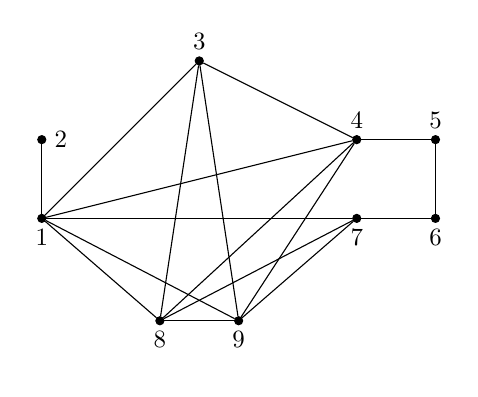
\begin{tikzpicture}[every node/.style={circle, inner sep=0.04cm, fill=black, draw, scale=0.9}, scale=1.0, rotate = 180, xscale = -1]

\node[label=below:{1}] (1) at ( 1, 4) {};
\node[label=right:{2}] (2) at ( 1, 3) {};
\node[label=above:{3}] (3) at ( 3, 2) {};
\node[label=above:{4}] (4) at ( 5., 3) {};
\node[label=above:{5}] (5) at ( 6, 3) {};
\node[label=below:{6}] (6) at ( 6, 4) {};
\node[label=below:{7}] (7) at ( 5, 4) {};
\node[label=below:{8}] (14) at ( 2.5, 5.3) {};
\node[label=below:{9}] (15) at ( 3.5, 5.3) {};

\draw (1) -- (2);
\draw (1) -- (3);
\draw (4) -- (3);
\draw (5) -- (4);
\draw (6) -- (5);
\draw (7) -- (6);
\draw (15) -- (7);
\draw (15) -- (4);
\draw (14) -- (7);
\draw (14) -- (4);
\draw (15) -- (3);
\draw (14) -- (3);
\draw (14) -- (1);
\draw (15) -- (1);
\draw (7) -- (1);
\draw (4) -- (1);
\draw (14) -- (15);
    \tikzstyle{empty}=[draw, shape=circle, minimum size=3pt,inner sep=0pt, fill=white,color=white]
\node[empty] () [below = 1.8cm] at (1) {};
\end{tikzpicture}
}
\quad
\scalebox{0.5}{
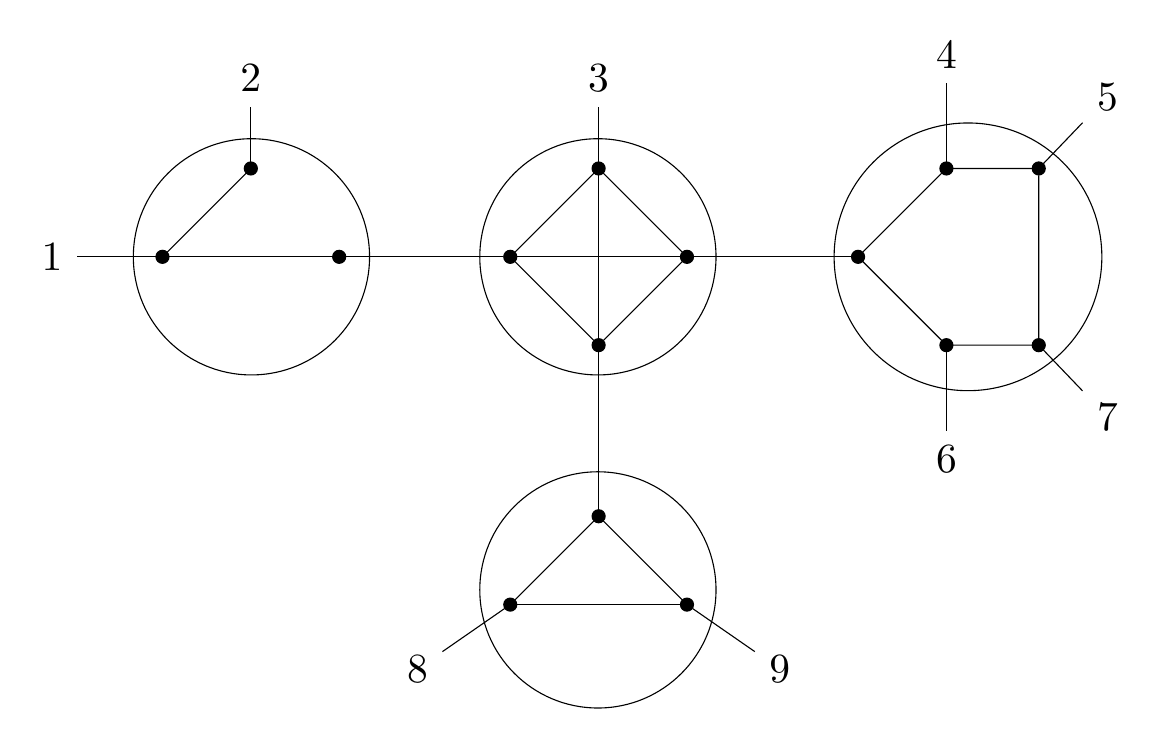
\begin{tikzpicture}[remember picture, 
outer/.style={ scale=1.5},
inner/.style= {circle, fill=black, draw, scale=.5},
scale=1.0, rotate = 180, xscale = -1]

		\node[inner] (a1) {};
		\node[inner, above right=of a1] (a2) {};
		\node[inner, below right=of a2] (a3) {};
        \node[below left=of a3] (a4) {};

		\draw (a1) -- (a2);
		\draw (a1) -- (a3);

		\node[inner, right=2cm of a3] (b1) {};
		\node[inner, above right=of b1] (b2) {};
		\node[inner, below right=of b2] (b3) {};
        \node[inner, below left=of b3] (b4) {};

		\draw (b1) -- (b2);
		\draw (b1) -- (b3);
		\draw (b1) -- (b4);
		\draw (b2) -- (b3);
		\draw (b2) -- (b4);
		\draw (b3) -- (b4);

		\node[inner, right= 2cm of b3] (c1) {};
		\node[inner, above right=of c1] (c2) {};
		\node[inner, below right=of c1] (c3) {};
        \node[inner, right=of c2] (c4) {};
        \node[inner, right=of c3] (c5) {};
        
        \draw (c1) -- (c2) -- (c4) -- (c5) -- (c3) -- (c1);

		\node[inner, below= 2cm of b4] (d1) {};
		\node[inner, below left=of d1] (d2) {};
		\node[inner, below right=of d1] (d3) {};

		\draw (d1) -- (d2);
		\draw (d1) -- (d3);
        \draw (d2) -- (d3);

\node[outer, left=1cm of a1] (1) {1};
\node[outer, above=0.7cm of a2] (2) {2};
\node[outer, above=0.7cm of b2] (3) {3};
\node[outer, above=1cm of c2] (4) {4};
\node[outer, above right=0.7cm of c4] (5) {5};
\node[outer, below=1cm of c3] (6) {6};
\node[outer, below right=0.7cm of c5] (7) {7};
\node[outer, below left=0.4cm and 0.8cm of d2] (8) {8};
\node[outer, below right=0.4cm and 0.8cm of d3] (9) {9};


\draw (a3) -- (b1);
\draw (b3) -- (c1);
\draw (b4) -- (d1);

 \draw (a1) -- (1);
 \draw (a2) -- (2);
 \draw (b2) -- (3);
 \draw (c2) -- (4);
 \draw (c4) -- (5);
 \draw (c3) -- (6);
 \draw (c5) -- (7);
 \draw (d2) -- (8);
 \draw (d3) -- (9);

\draw (1.13,0) circle (1.5cm);
\draw (5.53,0) circle (1.5cm);
\draw (10.23,0) circle (1.7cm);
\draw (5.53,4.23) circle (1.5cm);


\end{tikzpicture}
}
\end{center}
\caption{A graph-labeled tree (right) and its accessibility graph (left).}
\end{figure}

Two leaves are accessible if their associated marker vertices are accessible. The \emph{accessibility graph} of graph-labeled tree , denoted , is the graph whose vertices are leaves of  and which has an edge between two distinct leaves  and  if and only if they are accessible from one another. Conversely, we may say that  is the graph-labeled tree of .

\begin{definition}[\cite{GioanPaulTedderCorneil14}]
Let  be a tree-edge incident to internal nodes  and  in a \GLT, and let
 and  be the extremities of . The \emph{node-join} of ,  replaces 
and  with a new internal node  labeled by the graph formed from the disjoint union of  and  as
follows: all possible label-edges are added between  and , and then  and
 are deleted. The new node  is made adjacent to all neighbors of  and  in .
The \emph{node-split} is then the inverse of the node-join.
\end{definition}

Notice that the node-join operation and the node-split operation preserve the
accessibility graph of the GLT. A graph-labeled tree is \emph{reduced} if all its labels are either prime or degenerate, and no node-join of two cliques or two stars is possible.

\begin{theorem}[\cite{Cunningham82,GioanPaul07,GioanPaul12,GioanPaulTedderCorneil14}]\label{thm:uniquereducedGLT}
For any connected graph , there exists a unique, reduced graph-labeled tree  such that .
\end{theorem}

The unique \GLT~guaranteed by the previous theorem is the \emph{split-tree}, and is denoted .

\begin{theorem}[\cite{Cunningham82,GioanPaul07,GioanPaul12,GioanPaulTedderCorneil14}]\label{thm:splitinGLT}
Let    be the split-tree of a connected graph . Any split of  is the bipartition
(of leaves) induced by removing an internal tree-edge from , where  or  is
obtained from  by exactly one node-split of a degenerate node.
\end{theorem}


\begin{theorem}[\cite{GioanPaulTedderCorneil14}]\label{thm:computingGLT}
The split-tree  of a connected graph  with n vertices and
m edges can be built incrementally in time , where  is the inverse Ackermann function.
\end{theorem}
}

 \lv{\prelimsplitsb}

\paragraph{Rank-width}


For a graph  and , let  denote the
-submatrix of the adjacency matrix over the two-element
field , i.e., the entry ,  and , of  is  if and only if  is an edge
of~.  The {\em cut-rank} function  of a graph  is
defined as follows: For a bipartition  of the vertex
set~,  equals the rank of 
over . 

A \emph{rank-decomposition} of a graph  is a pair 
where  is a tree of maximum degree 3 and tT is a bijective function. For an edge~ of~, the connected components of  induce a
bipartition  of the set of leaves of~.  The \emph{width} of
an edge  of a rank-decomposition  is .
The \emph{width} of  is the maximum width over all edges of~.  The \emph{rank-width} of ,  in short, is the minimum width over all
rank-decompositions of . We denote by  the class of all graphs of rank-width at most , and say that a graph class  is of \emph{unbounded rank-width} if  for any .



\newenvironment{psmallmatrix}
  {\left(\begin{smallmatrix}}
  {\end{smallmatrix}\right)}

\begin{figure}[ht]
\vspace{-0.6cm}
\centering
  \tikzstyle{every circle node}=[circle,draw,inner sep=1.0pt, fill=black]
  \begin{tikzpicture}
    \begin{scope}[xshift=-7cm]
      \draw
      (90+4*72:1) node[circle] (d)  {} node[right=2pt] {} 
      (90+0*72:1) node[circle] (c)  {} node[above] {} 
      (90+1*72:1) node[circle] (b)  {} node[left=2pt] {} 
      (90+2*72:1) node[circle] (a)  {} node[below] {} 
      (90+3*72:1) node[circle] (e)  {} node[below] {} 
      (a)--(b)--(c)--(d)--(e)--(a)
      ;
    \end{scope}

 \draw 
 (-3,1)   node[circle] (d) {} node[above] {} 
 (-3,-1)  node[circle] (e) {} node[below] {} 
 (-2,0)   node[circle] (U) {} 
 (0,0)    node[circle] (V) {} 
 (0,-1.2)    node[circle] (X) {} node[below] {} 
 (2,0)    node[circle] (W) {}
 (3,1)   node[circle] (c) {} node[above] {} 
 (3,-1)  node[circle] (b) {} node[below] {} 

 (d) to node [auto,near start, swap] {} (U)
 (e) to node [auto, near start] {} (U)
 (U) to node [auto] {} (V)
 (V) to node [auto] {} (W)
 (V)  to node [auto] {} (X)
 (c)--(W)--(b)
(3.4,0.5) node {} 
(3.4,-0.5) node {} 
;
\end{tikzpicture}
\vspace{-0.8cm}
\caption{A rank-decomposition of the cycle .}
\label{fig:rdecC5}
\vspace{-0.6cm}
\end{figure}


\begin{theorem}[\cite{HlinenyOum08}]\label{thm:rankdecomp} Let  be a constant and
  . For an -vertex graph , we can output a
  rank-decomposition of width at most  or confirm that the
  rank-width of  is larger than  in time , where  is a computable function.
\end{theorem}

\paragraph{Monadic Second Order Logic on Graphs}
We assume that we have an infinite supply of individual variables,
denoted by lowercase letters , and an infinite supply of set
variables, denoted by uppercase letters . \emph{Formulas} of
\emph{monadic second-order logic} (MSO) are constructed from atomic
formulas , , and  using the connectives 
(negation),  (conjunction) and existential quantification
 over individual variables as well as existential
quantification  over set variables. Individual variables
range over vertices, and set variables range over sets of
vertices. The atomic formula  expresses adjacency, 
expresses equality, and  expresses that vertex  in the set
. From this, we define the semantics of monadic second-order logic
in the standard way (this logic is sometimes called ).

\emph{Free and bound variables} of a formula are defined in the usual way. A
\emph{sentence} is a formula without free variables. We write  to indicate that the set of free variables of formula 
is . If  is a graph and  we write  to denote that
 holds in  if the variables  are interpreted by the sets
, for . For a fixed \MSO sentence , the MSO Model Checking problem () asks whether an input graph  satisfies .

It is known that MSO formulas can be checked efficiently as long as the graph has bounded rank-width.

\begin{theorem}[\cite{GanianHlineny10}]\label{thm:msorankwidth}
  Let  and  be fixed
  \MSO formulas. Given an -vertex graph  and a set , there exists a computable function  such that we can decide whether  and whether  in time .
\end{theorem}

We review \MSO \emph{types} roughly following the presentation in
\cite{Libkin04}. The \emph{quantifier rank} of an \MSO formula  is
defined as the nesting depth of quantifiers in . For non\hy negative
integers  and , let  consist of all \MSO formulas of
quantifier rank at most  with free set variables in .

Let  and  be
\MSO formulas. We say  and  are \emph{equivalent}, written , if for all graphs  and ,  if and only if .  Given a set  of formulas, let  denote the set
of equivalence classes of  with respect to . A system of
representatives of  is a set  such that  for each equivalence class .
The following statement has a straightforward proof using normal forms (see
\cite[Proposition~7.5]{Libkin04} for details).
\begin{ourfact}\label{fact:representatives}
  Let  and  be fixed non\hy negative integers. The set
   is finite, and one can compute a system of
  representatives of .
\end{ourfact}
We will assume that for any pair of non\hy negative integers  and  the
system of representatives of  given by
Fact~\ref{fact:representatives} is fixed.
\begin{definition}[\MSO Type]
  Let  be non\hy negative integers. For a graph  and an \hy
  tuple  of sets of vertices of , we define
   as the set of formulas  such that . We call
   the \MSO \emph{-type of
     in }. 
\end{definition}
It follows from Fact~\ref{fact:representatives} that up to logical
equivalence, every type contains only finitely many formulas. \lv{This
allows us to represent types using \MSO formulas as follows.}

\newcommand{\lemtypeformula}[0]{
\begin{lemma}[\cite{GanianSlivovskySzeider13}]
\label{lem:typeformula}
  Let  and  be non\hy negative integer constants, let  be a graph,
  and let  be an \hy tuple of sets of vertices of . One can
  compute a formula  such that for any graph
   and any \hy tuple  of sets of vertices of  we have  if and only if . Moreover,  can be computed in time .
\end{lemma}

\begin{proof}
  Let  be a system of representatives of  given
  by Fact~\ref{fact:representatives}. Because  and  are constant, we can
  consider both the cardinality of  and the time required to compute it as
  constants. Let  be the formula defined as , where . We can compute  by deciding  for each . Since the number of formulas in
   is a constant, this can be done in time  if  can
  be decided in time .

  Let  be an arbitrary graph and let  be an \hy tuple of subsets of
  . We claim that  if and only if . Since  the forward direction is trivial. For the converse, assume
  . First
  suppose . The set  is a system of representatives
  of  , so there has to be a  such that
  . But  implies  by construction of  and thus , a contradiction. Now suppose . An
  analogous argument proves that there has to be a  such that
   and . It follows that
  , which again yields a contradiction.
  \qed
\end{proof}}
\lv{\lemtypeformula}

\newcommand{\MSOgames}[0]{
\begin{definition}[Partial isomorphism]\label{def:partialisomorphism}
  Let  be graphs, and let  and
   be tuples of sets of vertices with
   and  for each . Let  and  be tuples of vertices with  and 
  for each . Then  defines a
  \emph{partial isomorphism between  and } if the following conditions hold:
  \begin{itemize}
    \item For every ,
    
    \item For every  and ,
      
    \end{itemize}
\end{definition}

\begin{definition}
  Let  and  be graphs, and let  be a \hy tuple of subsets
  of  and let  be a \hy tuple of subsets of . Let
   be a non\hy negative integer. The \emph{\hy round \MSO game on 
    and  starting from } is played as follows.
  The game proceeds in rounds, and each round consists of one of the following
  kinds of moves.
\begin{itemize}
  \item \textbf{Point move} The Spoiler picks a vertex in either  or ; the Duplicator responds by picking a vertex in the other graph.
  \item \textbf{Set move} The Spoiler picks a subset of  or a
    subset of ; the Duplicator responds by picking a subset of the
    vertex set of the other graph.
  \end{itemize}
  Let  and  be the point
  moves played in the -round game, and let  and  be the set moves played in the
  \hy round game, so that  and moves belonging to same round
  have the same index. Then the Duplicator wins the game if  is a partial isomorphism of  and . If the Duplicator has a winning strategy, we write .
\end{definition}

\begin{theorem}[\cite{Libkin04}, Theorem 7.7]\label{thm:msogames} Given two graphs  and  and two \hy tuples  of sets of vertices of  and , we have 
\end{theorem}}

\lv{\MSOgames}


\section{Well-Structured Modulators}\label{sec:wsm}

\begin{definition}
\label{def:wsm}
Let  be a hereditary graph class and let  be a graph. A set  of pairwise-disjoint split-modules of  is called a -\emph{\wsm}{} to  if
\begin{enumerate}
\item , and
\item  is a modulator to , and
\item  for each .
\end{enumerate}
\end{definition}

\begin{figure}
\centering
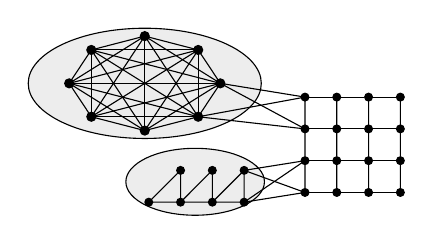
\begin{tikzpicture}[every node/.style={circle, fill=black, draw, scale=.3}, scale=0.5, rotate = 180, xscale = -0.8, yscale = 0.5]

\filldraw[fill opacity=0.7,fill=gray!20] (0,0) ellipse (3.7cm and 2.8cm);
\filldraw[fill opacity=0.7,fill=gray!20] (1.6,5) ellipse (2.2cm and 1.7cm);


 \foreach \x in {1,...,8}{\pgfmathparse{(\x-1)*45+floor(\x/9)*45}
    \node (N-\x) at (\pgfmathresult:2.4cm) [thick] {};
 } 
 \foreach \x [count=\xi from 1] in {2,...,8}{\foreach \y in {\x,...,8}{\path (N-\xi) edge[-] (N-\y);
  }
 }

 \newlength{\gridsize}
\setlength{\gridsize}{0.3cm}

\node[below right=0.1cm and 1cm of N-1] (1)  {};
\node[right=\gridsize of 1] (2) {};
\node[right=\gridsize of 2] (3) {};
\node[right=\gridsize of 3] (4) {};
\node[below=\gridsize of 1] (5) {};
\node[below=\gridsize of 2] (6) {};
\node[below=\gridsize of 3] (7) {};
\node[below=\gridsize of 4] (8) {};
\node[below=\gridsize of 5] (9) {};
\node[below=\gridsize of 6] (10) {};
\node[below=\gridsize of 7] (11) {};
\node[below=\gridsize of 8] (12) {};
\node[below=\gridsize of 9] (13) {};
\node[below=\gridsize of 10] (14) {};
\node[below=\gridsize of 11] (15) {};
\node[below=\gridsize of 12] (16) {};


\node[below left=0.05cm and 0.7cm of 13] (a1) {};
\node[below left=0.05cm and 0.7cm of 9] (a2) {};
\node[left=\gridsize of a1] (a3) {};
\node[left=\gridsize of a3] (a4) {};
\node[left=\gridsize of a2] (a5) {};
\node[left=\gridsize of a4] (a6) {};
\node[above=\gridsize of a4] (a7) {};


\draw (N-1)--(1)--(N-2);
\draw (N-2)--(5)--(N-1);
\draw (a3)--(a2)--(a1)--(a3)--(a4)--(a5)--(a3);
\draw (a4)--(a6)--(a7)--(a4);
\draw (a1)--(9)--(a2);
\draw (a1)--(13)--(a2);

\draw (1)--(2)--(3)--(4);
\draw (5)--(6)--(7)--(8);
\draw (9)--(10)--(11)--(12);
\draw (13)--(14)--(15)--(16);
\draw (1)--(5)--(9)--(13);
\draw (2)--(6)--(10)--(14);
\draw (3)--(7)--(11)--(15);
\draw (4)--(8)--(12)--(16);


\end{tikzpicture}
\caption{A graph with a -\wsm{} to -free graphs (in the two shaded areas)}
\vspace{-0.5cm}
\label{fig:wsm}
\end{figure}

For the sake of brevity and when clear from context, we will sometimes identify  with  (for instance  is shorthand for ). 
To allow a concise description of our parameters, for any hereditary graph class  we let the \emph{well-structure number} ( in short) denote the minimum  such that  has a -{\wsm} to . Similarly, we let  denote the minimum  such that~ has a modulator of cardinality  to . 

\sv{\begin{proposition}}
\lv{\begin{proposition}}
\label{prop:better}
Let  be \emph{any} hereditary graph class of unbounded rank-width.
\begin{enumerate}
\item  for any graph . Furthermore, for every  there exists a graph  such that , and
\item  for any graph . Furthermore, for every  there exists a graph  such that .
\end{enumerate}
\end{proposition}

\newcommand{\pfpropbetter}[0]{
\begin{proof}
\begin{enumerate}
\item For  notice that for any graph  of rank-width , the set  is a -{\wsm} to the empty graph. For the second claim, since  has unbounded rank-width, for every  it contains some graph  such that ; by definition, .
\item For , let  be a graph containing a modulator   to . It is easy to check that  is a -{\wsm} to . For the second claim, let  and let . Consider the graph  consisting of  disjoint copies of  and a vertex  which is adjacent to every other vertex of . Since  is hereditary, we may assume without loss of generality that it contains the single-vertex graph. It is then easy to check that  forms a -{\wsm} in  to . Now consider any set  of cardinality at most . Clearly, there must exist some copy of , say , such that . Since , it follows from the hereditarity of  that  and hence  cannot be a modulator to . We conclude .
\qed
\end{enumerate}
\end{proof}}

\lv{\pfpropbetter}




\section{Finding Well-Structured Modulators}
\label{sec:finding}

The objective of this subsection is to prove the following theorem. Interestingly, our approach only allows us to find \wsm s if the rank-width of the graph is sufficiently large. This never becomes a problem though, since on graphs with small rank-width we can always directly use rank-width as our parameter.\sv{\enlargethispage*{8mm}}

\begin{theorem}
\label{thm:main-find}
Let  be a graph class characterized by a finite obstruction set. There exists an \emph{FPT} algorithm parameterized by  which for any graph  of rank-width at least  either finds a -{\wsm} to  or correctly detects that it does not exist. 
\end{theorem}

\lsv{
We begin by stating several useful properties of splits in graphs. We remark that for most of this section we will restrict ourselves to connected graphs, and show how to deal with general graphs later on; this allows us to use the following result by Cunningham.}
{Our starting point on the path to a proof of Theorem~\ref{thm:main-find} is a theorem by Cunningham.}

\begin{theorem}[\cite{Cunningham82}]\label{thm:splitintersection}
Let ,  be splits of a connected graph  such that   and
. Then  is a split of .
\end{theorem}

\newcommand{\lemunion}[0]{
\begin{lemma}\label{lem:smintersection}
If  and  are overlapping \sm\-s of a connected graph , then  is also a \sm. Moreover, if , then also  is a \sm.
\end{lemma}

\begin{proof}
If , then  is clearly a \sm. 
So, assume  and let  and ; note that  since  are overlapping. We make the following exhaustive case distinction:
\begin{itemize}
\item if  and , then both  and  are easily seen to be \sm s;
\item if  and , then  is a {\sm} by Theorem~\ref{thm:splitintersection} and  is also a {\sm} because  is a {\sm};
\item if  and , then  is a {\sm} and  is also a {\sm} because  satisfy the conditions of Theorem~\ref{thm:splitintersection} and hence  forms a \sm;
\item if  and , then  is a {\sm} by Theorem~\ref{thm:splitintersection} and  is also a {\sm} because  satisfy the conditions of Theorem~\ref{thm:splitintersection}, as in the previous case.
\end{itemize}
\vspace{-0.7cm}
\qed
\end{proof}

\begin{lemma}\label{lem:diferrence}
Let  be a connected graph and  be overlapping \sm s. Then  is also a \sm. 
\end{lemma}

\begin{proof}
The lemma clearly holds if , so we may assume that .
Let ; since  is a split module, so is . Furthermore, since  and  are overlapping, it holds that  is nonempty and hence . Since , we have  and hence we conclude that  is a split module by Theorem~\ref{thm:splitintersection}.
\qed
 \end{proof}

\begin{lemma}\label{lem:unionrw}
Let  be a constant,  a graph, and  , ,  be pairwise disjoint \sm s such that . Let , ,  be arbitrary vertices such that , , and . 
If , then .
\end{lemma}

\begin{proof}
Let
  , , and 
 be witnessing rank
  decompositions of , and ,
 respectively.
 
 We construct a rank decomposition  of  as follows.  
 
 Let  be the leaf (note that  is
 bijective) of  such that . 
Similarly, let  and  be the leaves such that  and , respectively.  
 We obtain  from  by adding disjoint copies of
  and  and then identifying  with the copies of
  and . Since , and  are subcubic, so
 is .
 
 We define the mapping  t
 is a leaf of  by
  
  where  maps internal nodes in  to their copies in
  . The mappings , and  are
  bijections and  is injective, so  is injective. By
  construction, the image of  under  is the set of
  leaves of , so  is a bijection. Thus  is a rank decomposition of .

We prove that the width of  is at most . Given a rank
  decomposition  and an edge  of , the
  connected components of  induce a bipartition 
  of the leaves of . We set . Take any edge  of . There is a
  natural bijection  from the edges in  to the edges of . Accordingly, we distinguish three cases for :
 
  \begin{enumerate}
  \item . Let . Without loss of generality assume that .  Then by construction of  , we have . Let  and . Since  is \sm~either  and  for all , or  in which case  for all . Therefore, to obtain  one can simply copy the column corresponding to  in  or add some empty columns. This does not increase the rank of the matrix. \label{rwmodule:case1}
  \item . This case is symmetric to case~\ref{rwmodule:case1}, with
     and  switching their roles and   taking the role of .
  \item . This case is symmetric to case~\ref{rwmodule:case1}, with
     and  switching their roles and   taking the role of .
  \end{enumerate}
  Since  is bijective, this proves that the rank of any bipartite
  adjacency matrix induced by removing an edge  is bounded by . We
  conclude that the width of  is at most  and thus
  \mbox{}.
  \qed
\end{proof}

By repeating the proof technique of Lemma~\ref{lem:unionrw} without the set , we obtain the following corollary.
\begin{corollary}
\label{cor:justtwosets}
Let  be a constant,  a graph, and  ,  pairwise disjoint \sm s such that . Let  be such that  and . 
If , then .
\end{corollary}

\begin{lemma}\label{lem:smallrw}
 Let  be a constant. Let  be a connected graph and let 
  be \sm s of  such that  and . Then .
\end{lemma}

\begin{proof}
Let . Clearly,  is a split. Since rank-width is preserved by taking induced subgraphs, the graph  has rank-width at most . Let  and . It is easy to see that 
graphs   and  have rank-width at most
 . We finish the proof by applying Corollary~\ref{cor:justtwosets}, with , 
 in roles of ,  and ,  in roles of , , respectively.
 \qed
\end{proof}}
\lv{\lemunion}

The following lemma in essence shows that the relation of being in a split-module of small rank-width is transitive (assuming sufficiently high rank-width). The significance of this will become clear later on.
\sv{\begin{lemma}}
\lv{\begin{lemma}}
\label{lem:union}
  Let  be a constant. Let  be a connected graph with rank-width at least  and let 
  be {\sm s} of  such that  and . Then  is a {\sm} of  and .
\end{lemma}

\newcommand{\pflemunion}[0]{
\begin{proof}
  If  or  the result is
  immediate, hence we may assume that they are overlapping.
  Lemma~\ref{lem:smallrw} and  together imply that .
Let
  , and
 . It follows from Lemma~\ref{lem:smintersection} and Lemma~\ref{lem:diferrence} that these
  sets are {\sm s} of . Let , and
  . We show that . By
  assumption, both
  and  have rank-width at most . Since
  rank-width
 is preserved by taking induced subgraphs, the graphs , ,
 and
   also have rank-width at most
 . We finish the proof by applying Lemma~\ref{lem:unionrw}, with , , 
 taking the roles of , , and  and , , and  taking the roles of , , and , respectively. 
 \qed
\end{proof}}

\lv{\pflemunion}

\sv{
\begin{proof}[Sketch]
The proof relies on a series of lemmas building on Theorem~\ref{thm:splitintersection}. 

  If  or  the result is
  immediate, hence we may assume that they are overlapping.
   implies that . The fact that  is a {\sm} of  then follows from Theorem~\ref{thm:splitintersection}. Let
  , and
 . These sets can be shown to be {\sm s} of . Let , and
  . We show that . By
  assumption, both
  and  have rank-width at most . Since
  rank-width
 is preserved by taking induced subgraphs, the graphs , ,
 and
   also have rank-width at most
 . The proof can be completed by showing how the rank-decompositions of these three graphs can be combined into a rank-decomposition for .
\qed
\end{proof}
}
\begin{definition}
  Let  be a graph and .  We define a relation
   on  by letting  if and only if there
  is a {\sm}  of  with  and . We
  drop the superscript from  if the graph  is clear from
  context.
\end{definition}

Using Lemma~\ref{lem:union} to deal with transitivity, we prove the following.
\lv{\begin{proposition}}
\sv{\begin{proposition}}
\label{prop:eqrel}
  For every  and graph  with rank-width at least , the relation  is an
  equivalence relation, and each equivalence class  of  is a {\sm}
  of  with .\end{proposition}

\newcommand{\pfpropeqrel}[0]{
\begin{proof} 
  Let  be a graph and . For every , the
  singleton  is a {\sm} of , so  is reflexive. Symmetry of
   is trivial. For transitivity, let  be such that  and . Then there are {\sm s}  of  such
  that , , and ; in particular, since  this implies that there exists a connected component  of  containing . By
  Lemma~\ref{lem:union},  is a {\sm} of  (and hence also of ) such that . In combination with  that implies . This concludes the proof that  is an equivalence
  relation.
  
  Now let ,  be the connected component containing , and let . For each  there is
  a {\sm}  of  (and of ) with  and . By
  Lemma~\ref{lem:union},  is a {\sm} of  (and hence also of ) and . Clearly, . On the other hand,
   implies  by definition of , so . That is, .
\end{proof}}
\lv{\pfpropeqrel}

\begin{corollary}
\label{cor:equiv}
Any graph  of rank-width at least  has its vertex set uniquely partitioned by the equivalence classes of  into inclusion-maximal \sm s of rank-width at most .
\end{corollary}

\lv{Next, we state a simple but useful observation.}

\newcommand{\obsdisconequiv}[0]{
\begin{observation}
\label{obs:disconequiv}
Let ,  be a disconnected graph with rank-width at least , and  be the set of connected components of . Then .
\end{observation}
}
\lv{\obsdisconequiv}

Now that we know  is an equivalence, we show how to compute it in FPT time.

\lv{\begin{proposition}}
\sv{\begin{proposition}}
\label{prop:equdecision}
  Let  be a constant. Given an -vertex graph  of rank-width at least  and two vertices , we can decide whether  in time .
\end{proposition}

\newcommand{\pfpropequdecision}[0]{
\begin{proof}
From Observation~\ref{obs:disconequiv} it follows that if the proposition holds for connected graphs, then it holds for disconnected graphs as well; hence we may assume that  is connected. By Theorem~\ref{thm:computingGLT} we can compute the unique split-tree  in 
 time. Due to Theorem~\ref{thm:splitinGLT}, every split in  is the bipartition of leaves of  induced either by removing an internal tree-edge of  or an edge created by a node-split of a degenerate vertex of . 

Vertices of  are leaves of  and we can find a path  between  and  in  in time linear in size of . There are at most linearly many vertices on the path and we can split every degenerate vertex on  in a way that every degenerate vertex on a new path  between  and  will have  vertices. Denote the new tree by .

Now every edge between  and  corresponds to a minimal \sm~containing  and . Conversely, as a consequence of Theorem~\ref{thm:splitinGLT} every minimal {\sm} containing  and  is induced by removing an edge between  and , and let  be the set containing all of these at most  minimal split modules. Hence,  if and only if there is a {\sm}  in  such that .
By Theorem~\ref{thm:rankdecomp} we can decide, for each such , whether  in time , where  is some computable function.
\qed
\end{proof}}

\lv{\pfpropequdecision}

\sv{\begin{proof}[Sketch]
The definition of \sm s allows us to consider each connected component of a graph separately. We then compute the so-called \emph{split-tree}~\cite{Cunningham82,GioanPaul07,GioanPaul12,GioanPaulTedderCorneil14} of  and use it to list all minimal \sm s containing  and . Finally, we check whether any of these \sm s has rank-width at most  by using Theorem~\ref{thm:rankdecomp}.
\qed
\end{proof}
}

\lv{In the rest of this section we show how to find a -\wsm{} to any graph class  characterized by a finite obstruction set . We first present the algorithm and then show its running time and correctness.}
\sv{We are now ready to present an algorithm for finding a -\wsm{} to any graph class  characterized by a finite obstruction set .}

\medskip
\RestyleAlgo{boxruled}
\begin{algorithm}[H]
\LinesNumbered

\SetKwInOut{Input}{Input}\SetKwInOut{Output}{Output}
\SetKwInOut{Parameter}{Parameter}

 \Input{, -vertex graph , equivalence  over a superset of }
\Output{A -cardinality set  of subsets of , or \emph{False}}



\BlankLine
  \uIf{ does not contain any  as an induced subgraph}{\KwRet{}}
  \Else{ an induced subgraph of  isomorphic to an arbitrary \;}
 \lIf{}{\KwRet{False}}


\ForEach{ of  which intersects with }{
	\;\label{algstep:recursion}
	\If{ \emph{False}}{
	\KwRet{}	
	}
}

\KwRet{False}
 \caption{FindWSM} \label{alg:findingmodulator}
\end{algorithm}
 \medskip
 
We will use  as the input for \emph{FindWSM}, however considering general equivalences as inputs is useful for proving correctness.
\lv{Recall that the equivalence  (or, more precisely, the set of its equivalence classes) can be computed in time  for some function  thanks to Proposition~\ref{prop:equdecision}, and this only needs to be done once before starting the algorithm.} \lv{The following two lemmas show that Algorithm~\ref{alg:findingmodulator} is correct and runs in FPT time.}

\sv{
\begin{lemma}
\label{lem:algo}
There exists a constant  such that \emph{FindWSM} runs in time . Furthermore, if  is a graph of rank-width at least  and  is the equivalence computed by Proposition~\ref{prop:equdecision}, then \emph{FindWSM} outputs a -wsm{} to  or correctly detects that no such -wsm exists in .
\end{lemma}
}

\newcommand{\algo}[0]{
\begin{lemma}
\label{lem:algoruntime}
There exists a constant  such that \emph{FindWSM} runs in time .
\end{lemma}
\begin{proof}
The time required to perform the steps on rows {-} is  since  is finite. For the same reason, it holds that  and hence also the number of times the procedure on rows {-} is called are bounded by a constant, say  (to be precise,  is bounded by the order of the largest graph in ). 

For the rest of the proof, we proceed by induction on .
First, if , then the algorithm is polynomial by the above. So assume that  and the algorithm for  runs in time at most . Then the algorithm for  will run in polynomial time up to rows {}, where it will make at most  calls to the algorithm for , which implies that the running time for  is bounded by . \qed
\end{proof}

\begin{lemma}
\label{lem:algocorrect}
Let ,  be a graph and  an equivalence over a superset of . Then
\emph{FindWSM} outputs a set  of at most  equivalence classes of  such that  is -free. 
\end{lemma}

\begin{proof}
If  does not contain any  as an induced subgraph, then we correctly return the empty set. So, assume there exists an induced subgraph  of  isomorphic to .  
We prove the lemma by induction on . 

Clearly, if  but there exists some obstruction, then the algorithm outputs \emph{False} and this is correct; if  and no obstruction exists, then the algorithm correctly outputs . 
Let  and assume that the algorithm is correct for . If  does not contain any such , then for any equivalence class , FindWSM will correctly output \emph{False}. 

On the other hand, assume  does contain some  with the desired properties. In particular, this implies that  must intersect . Let  be an arbitrary equivalence class of  which intersects . Then  is a set of at most  equivalence classes of  in , and hence FindWSM will output some solution  for  by our inductive assumption. Since any obstruction in  intersecting  is removed by  and  is made -free by , we observe that  intersects every obstruction in  and hence the proof is complete.
\qed
\end{proof}

From Lemma~\ref{lem:algocorrect} and Corollary~\ref{cor:equiv} we obtain the following.
 
\begin{corollary}
\label{cor:algocorrect}
Let ,  be a graph of rank-width at least  and  be the equivalence computed by Proposition~\ref{prop:equdecision}. Then
\emph{FindWSM} outputs a -wsm{} to  or correctly detects that no such -wsm exists in .
\end{corollary}}

\lv{\algo}

\begin{proof}[of Theorem~\ref{thm:main-find}]
\lv{The theorem follows by using Proposition~\ref{prop:equdecision} and then Algorithm~\ref{alg:findingmodulator} in conjunction with Lemma~\ref{lem:algoruntime} and~\ref{lem:algocorrect}.}
\sv{The theorem follows by using Proposition~\ref{prop:equdecision} and then Algorithm~\ref{alg:findingmodulator} in conjunction with Lemma~\ref{lem:algo}.}
\qed
\end{proof}





\section{Examples of Algorithmic Applications}
\label{sec:examples}

In this section, we show how to use the notion of -\wsm s to design efficient parameterized algorithms for two classical NP-hard graph problems, specifically \textsc{Minimum Vertex Cover (MinVC)} and \textsc{Maximum Clique (MaxClq)}. Given a graph , we call a set  a \emph{vertex cover} if every edge is incident to at least one  and a \emph{clique} if  is a complete graph.

\vspace{-.5cm}
\begin{center}
  \begin{boxedminipage}[t]{0.99\textwidth}
\begin{quote}
\smallskip
  \textsc{MinVC, MaxClq}\\ \nopagebreak
\emph{Instance}: A graph  and an integer .\\ \nopagebreak
  \emph{Task} (\textsc{MinVC}): Find a vertex cover in  of cardinality at most , or determine that it does not exist. \\
\emph{Task} (\textsc{MaxClq}): Find a clique in  of cardinality at least , or determine that it does not exist. \smallskip
\end{quote}
\end{boxedminipage}
\end{center}

Establishing the following theorem is the main objective of this section.

\begin{theorem}
\label{thm:problems}
Let  and  be a graph class characterized by a finite obstruction set. Then  is \emph{FPT} parameterized by  if and only if  is polynomial-time tractable on .
\end{theorem}

Since  for any -free graph , the ``only if'' direction is immediate; in other words, being polynomial-time tractable on  is clearly a necessary condition for being fixed parameter tractable when parameterized by . Below we prove that for the selected problems this condition is also sufficient.

\lv{\begin{lemma}}
\sv{\begin{lemma}}
\label{lem:vc}
If \textsc{MinVC} is polynomial-time tractable on a graph class  characterized by a finite obstruction set, then  is \emph{FPT}.
\end{lemma}

\newcommand{\pflemvc}[0]{
\begin{proof}
Let  be a graph and let . If , then we simply use known algorithms to solve the problem in FPT time~\cite{GanianHlineny10}. Otherwise, we proceed by using Theorem~\ref{thm:main-find} to compute a -{\wsm}  in FPT time. For each , we let  be the frontier of  and we let .

Since for each  the graph  contains a complete bipartite graph, any vertex cover of  must be a superset of either  or . We can branch over these options for each  in  time; formally, we branch over all of the at most  functions , and refer to these as \emph{signatures}. Each vertex cover  of  can be associated with at least one signature , constructed in the following way: for each  such that , we set , and otherwise we set .

Our algorithm then proceeds as follows. For a graph  and a signature , we construct a partial vertex cover . We let . Consider any connected component  of . If  intersects some , then by the construction of  it must hold that . Hence it follows that  either has rank-width at most  (in the case  for some ), or  is in  (if  does not intersect ), or both. Then we find a minimum vertex cover for each connected component of  independently, by either calling the known FPT algorithm (if  has bounded rank-width) or the polynomial algorithm (if  is in ) at most  times. Let  be the union of the obtained minimum vertex covers over all the components of , and let . After branching over all possible functions , we compare the obtained cardinalities of  and choose any  of minimum cardinality. Finally, we compare  and the value of  provided in the input.

We argue correctness in two steps. First, assume for a contradiction that  contains an edge  which is not covered by  for some . Then  cannot have both endpoints in , since  contains a (minimum) vertex cover for each connected component of , but  cannot have an endpoint outside of , since . Hence each  is a vertex cover of .

Second, assume for a contradiction that there exists a vertex cover  of  which has a lower cardinality than the vertex cover found by the algorithm described above. Let  be the signature of . Then it follows that , and since , there would exist a component  of  such that . However, this would contradict the minimality of . Hence we conclude that no such  can exist, and the algorithm is correct.
\qed
\end{proof}}
\lv{\pflemvc}

\sv{\begin{proof}[Sketch]
We compute a -\wsm{}  to  in  by Theorem~\ref{thm:main-find}. For each element , it holds that either the frontier of  or its neighborhood in  must be in any vertex cover of . Branching on these at most  options allows us to reduce the instance to at most  disconnected instances such that each connected component has either rank-width bounded by  or is in ; these connected components can then be solved independently.
\qed
\end{proof}
}





\lv{We deal with the second problem below.}

\sv{\begin{lemma}}
\lv{\begin{lemma}}
\label{lem:clq}
If \textsc{MaxClq} is polynomial-time tractable on a graph class  characterized by a finite obstruction set, then  is \emph{FPT}.
\end{lemma}

\newcommand{\pflemclq}[0]{
\begin{proof}
We begin in the same way as for \textsc{MinVC}: let  be a graph and let . If , then we simply use known algorithms to solve the problem in FPT time~\cite{GanianHlineny10}. Otherwise, we proceed by using Theorem~\ref{thm:main-find} to compute a -{\wsm}  in FPT time. For each , we let  be the frontier of  and we let .

Let  and let . Then any clique  in  can be uniquely associated with a \emph{signature}  by letting  if and only if . The algorithm proceeds by branching over all of the at most  possible non-empty signatures . If , then the algorithm simply computes a maximum-cardinality clique in  (by calling the respective FPT or polynomial algorithm at most a linear number of times) and stores it as . 

If , then the algorithm makes two checks before proceeding. First, if  then it constructs the set  of all vertices  such that  is adjacent to every  for . If  then the current choice of  is discarded and the algorithm proceeds to the next choice of . Second, for every  such that  it checks that  and  are adjacent; again, if this is not the case, then we discard this choice of  and proceed to the next choice of . Finally, if the current choice of  passed both tests then for each  we compute a maximum clique in each  and save their union as . In the end, we choose a maximum-cardinality set  and compare its cardinality to the value of  provided in the input.

We again argue correctness in two steps. First, assume for a contradiction that  is not a clique, i.e., there exist distinct non-adjacent . Since  consists of a union of cliques within subsets of , it follows that there would have to exist distinct  such that  and . This can however be ruled out for  or  equal to  by the construction of . Similarly, if  and  are both non-zero, then this is impossible by the second check which tests adjacency of every pair of  and  for every .

Second, assume for a contradiction that there exists a clique  in  which has a higher cardinality than the largest clique obtained by the above algorithm. Let  be the signature of . If  then  by the correctness of the respective FPT or polynomial algorithm used for each . If  then  may only intersect the sets  constructed above for . Moreover, if there exists  such that  then we again arrive at a contradiction with the correctness of the respective FPT or polynomial algorithms used for . Hence we conclude that no such  can exist, and the algorithm is correct.
\qed
\end{proof}}
\lv{\pflemclq}

Finally, let us review some concrete graph classes for use in Theorem~\ref{thm:problems}.
\lv{We use ,  and  to denote the -vertex complete graph, cycle, and path, respectively.  denotes the disjoint union of two  graphs, and the \emph{fork} graph is depicted for instance in~\cite{Alekseev04}. The , \emph{banner}, \emph{twin-house} and  graphs are defined in~\cite{BrandstadtLozin01,GerberLozin03}.}

\sv{\begin{ourfact}}
\lv{\begin{ourfact}}
  \label{fact:vcistract}
\textsc{MinVC} is polynomial-time tractable on the following graph classes:
\begin{enumerate}
\item -free graphs (split graphs);
\item -free graphs\sv{~{\normalfont\cite{LokshtanovVatshelleVillanger14}}};
\item fork-free graphs\sv{~{\normalfont\cite{Alekseev04}}};
\item -free graphs and -free graphs\sv{~{\normalfont\cite{GerberLozin03,BrandstadtLozin01}}}.
\end{enumerate}
\end{ourfact}

\newcommand{\pffactvcistract}[0]{
\begin{proof}
\begin{enumerate}
\item Split graphs are graphs whose vertex set can be partitioned into one clique and one independent set, and this partitioning can be found in linear time. If each vertex in the clique is adjacent to at least one independent vertex, then the clique is a minimum vertex cover, otherwise the clique without a pendant-free vertex is a minimum vertex cover.
\item See \cite{LokshtanovVatshelleVillanger14}.
\item See \cite{Alekseev04}.
\item See \cite{GerberLozin03} and \cite{BrandstadtLozin01}. \qed
\end{enumerate}
\end{proof}}
\lv{\pffactvcistract}

\sv{\begin{ourfact}}
\lv{\begin{ourfact}}
\label{fact:clqistract}
\textsc{MaxClq} is polynomial-time tractable on the following graph classes:
\begin{enumerate}
\item Any complementary graph class to the classes listed in Fact \ref{fact:vcistract} (such as cofork-free graphs and split graphs);
\item Graphs of bounded degree.
\end{enumerate}
\end{ourfact}

\newcommand{\pffactclqistract}[0]{
\begin{proof}
\begin{enumerate}
\item It is well-known that each maximum clique corresponds to a maximum independent set (and vice-versa) in the complement graph.
\item The degree bounds the size of a maximum clique, again resulting in a simple folklore branching algorithm. The class of graphs of degree at most  is exactly the class of -free graphs for  containing all -vertex supergraphs of the star with  leaves. \qed
\end{enumerate}
\end{proof}}
\lv{\pffactclqistract}




\section{ Model Checking with Well-Structured Modulators}
\label{sec:mso}

Here we show how well-structured modulators can be used to solve the MSO Model Checking problem, as formalized in Theorem~\ref{thm:main-use} below.
Note that our meta-theorem captures not only the generality of MSO model checking problems, but also applies to a potentially unbounded number of choices of the graph class . Thus, the meta-theorem supports two dimensions of generality.

\begin{theorem}\label{thm:main-use}
For every  sentence  and every graph class  characterized by a finite obstruction set such that  is \emph{FPT} parameterized by , the problem  is \emph{FPT} parameterized by .
\end{theorem}
The condition that  is FPT parameterized by  is a necessary condition for the theorem to hold by Proposition~\ref{prop:better}. However, it is natural to ask whether it is possible to use a weaker necessary condition instead, specifically that  is polynomial-time tractable in the class of -free graphs (as was done for specific problems in Section~\ref{sec:examples}). Before proceeding towards a proof of Theorem~\ref{thm:main-use}, we make a digression and show that the weaker condition used in Theorem~\ref{thm:problems} is in fact not sufficient for the general case of MSO model checking. 


\lv{\begin{lemma}}
\sv{\begin{lemma}}
\label{lem:MSOhard}
There exists an MSO sentence  and a graph class  characterized by a finite obstruction set such that  is polynomial-time tractable on  but NP-hard on the class of graphs with  or even .
\end{lemma}

\newcommand{\pflemMSOhard}[0]{
\begin{proof}
Consider the sentence  which describes the existence of a proper -coloring of the vertices of , and let  be the class of graphs of degree at most  (in other words, let  contain all -vertex supergraphs of the star with  leaves). There exists a trivial greedy algorithm to obtain a proper -coloring of any graph of degree at most , hence  is polynomial-time tractable on . Now consider the class of graphs obtained from  by adding, to any graph in , two adjacent vertices  which are both adjacent to every other vertex in the graph. By construction, any graph  from this new class satisfies  and hence also . However,  admits a proper -coloring if and only if  admits a proper -coloring. Testing -colorability on graphs of degree at most  is known to be NP-hard~\cite{KocholLozinRanderath03}, and hence the proof is complete.
\qed
\end{proof}}
\lv{\pflemMSOhard}

\sv{\begin{proof}[Sketch]
Let  describe vertex -colorability and let  be the class of graphs of degree at most . Now consider the class of graphs obtained from  by adding two adjacent vertices  which are adjacent to every other vertex. Hardness follows from hardness of -colorability on graphs of degree at most ~\cite{KocholLozinRanderath03}.
\qed
\end{proof}
}

Our strategy for proving Theorem~\ref{thm:main-use} relies on a replacement technique, where each split-module in the \wsm{} is replaced by a small representative. We use the notion of \emph{similarity} defined below to prove that this procedure does not change the outcome of \MSOMC{\varphi}.

\begin{definition}[Similarity]\label{def:similarity}
  Let  and  be non\hy negative integers,  be a graph class, and let  and  be graphs with -\wsm s  and  to ,
  respectively. For , let  contain the frontier of split module  and similarly let  contain the frontier of split module .
We say that  and  are \emph{-similar}
  if all of the following conditions are met:
  \begin{enumerate}
  \item There exists an isomorphism  between  and . \label{cond:sameH}
  \item For every  and , it holds that  is adjacent to  if and only if  is adjacent to .\label{cond:Hcon}
  \item if , then for every  it holds that  and  are adjacent if and only if  and  are adjacent. \label{cond:splitcon}
  \item For each , it holds that . \label{cond:sametypes}
\end{enumerate}
\end{definition}

\lv{\begin{lemma}}
\sv{\begin{lemma}}
\label{lem:partitiongame}
  Let  and  be non\hy negative integers,  be a graph class, and let  and  be graphs with -\wsm s 
   and  to ,
  respectively. If  and  are \emph{-similar}, then 
  .
  \end{lemma}
  
\newcommand{\pflempartitiongame}[0]{
\begin{proof}
  For , we write  and . Let  and . By Theorem~\ref{thm:msogames}, Condition~\ref{cond:sametypes} of
  Definition~\ref{def:similarity} is equivalent to . That is, for each ,
  Duplicator has a winning strategy  in the \hy round \MSO game
  played on  and  starting from . We
  construct a strategy witnessing  in the following way:
    \begin{enumerate}
    \item Suppose Spoiler makes a set move  and assume without loss of
      generality that . For , let , and let  be Duplicator's response to  according to
      . Furthermore, let . Then Duplicator responds with .
    \item Suppose Spoiler makes a point move  and again assume without loss
      of generality that . If  for some , then Duplicator responds with  according to ; otherwise, Duplicator responds with  as per Definition~\ref{def:similarity} point~\ref{cond:sameH}.
    \end{enumerate}
    Assume Duplicator plays according to this strategy and consider a play of
    the \hy round \MSO game on  and  starting from . Let  and
     be the point moves in  and  respectively, and let  and  be the set
    moves in  and  respectively, so that  and the moves made in the same round have the same index. We claim that 
    defines a partial isomorphism between  and .
\begin{itemize}
    \item Let  and let . Since  is an isomorphism as per Definition~\ref{def:similarity} point~\ref{cond:sameH}, it follows that  if and only if  and  if and only if .
    
    \item Let  and let  be such that  and . Then clearly  and . Consider the case . Then  must lie in the frontier of , and hence . Since Duplicator's strategy  is winning for  and , it must hold that . By Definition~\ref{def:similarity} point~\ref{cond:Hcon}, it then follows that . So, consider the case . Then either , in which case it holds that  because of the choice of  and hence there cannot be an edge  in , or , in which case it holds once again that  by Definition~\ref{def:similarity} point~\ref{cond:Hcon}.
    
    \item Let  and let  be such that . Since
      Duplicator plays according to a winning strategy  in the game on 
      and , the restriction  defines a partial
      isomorphism between  and . It follows that  if
      and only if  and  if and
      only if .  
    
      \item Let  and let  be pairwise distinct numbers such that  and . Then  and also  since  and  by the Duplicator's strategy. Suppose . Then , and , and  and  are adjacent in . From the correctness of  and  it follows that  and , and from Definition~\ref{def:similarity} point~\ref{cond:splitcon} it follows that  and  are adjacent in , which together implies  . On the other hand, suppose . Then either , or , or  and  are not adjacent in . In the first case we have , in the second case we have , and in the third case it holds that  and  are not adjacent in ; any of these three cases imply .
    
    \item Let  such that . Then by the Duplicator's strategy on  it follows that for any  such that  it holds that  and for any  such that  it holds that .
    
    \item Let  and  such that . Let  be such that . Since  is a winning strategy for Duplicator, it must be the case that . Similarly, if  then the correctness of  guarantetes that .\qed
  \end{itemize}
\end{proof}}

\lv{\pflempartitiongame}

\sv{
\begin{proof}[Sketch]
The proof argument uses the -round MSO game defined, e.g., in~\cite{Libkin04}. The notion of -similarity ensures that the Duplicator has a winning strategy on , which translates to  and  having the same . If the Spoiler moves in , then the Duplicator can follow the winning strategies for each . On the other hand, if the Spoiler moves in , then the Duplicator can copy this move in .
\qed
\end{proof}
}

\lv{Next, we show that small representatives can be computed efficiently.}

\newcommand{\lemconstantrep}[0]{
\begin{lemma}
\label{lem:constantrep} Let  be a non\hy negative integer
  constant. Let  be a graph of rank-width at most  and . Then there exists a function  such that one can in time  compute a graph  and a set  such that
   is bounded by a constant and .
\end{lemma}

\begin{proof}
  By Lemma~\ref{lem:typeformula} we can compute a formula  capturing the
  type  of  in time . Given , a constant-size model 
  satisfying  can be computed as follows. We start enumerating all graphs (by brute force and in any order with a non-decreasing number of vertices),
  and check for each graph  and every vertex-subset  whether . If this is
  the case, we stop and output . Since  this procedure
  must terminate eventually. Fixing the order in which graphs are
  enumerated, the number of graphs we have to check depends only on . By
  Fact~\ref{fact:representatives} the number of \hy types is finite
  for each , so we can think of the total number of checks and the size of each checked graph  as bounded by a constant. Moreover the time spent on each check depends only on  and the size of the graph . Consequently, after we compute  it is possible to find a model for  in constant time.
  \qed
\end{proof}}

\lv{\lemconstantrep}

\lv{Finally, in Lemma~\ref{lem:similar} below we use Lemma \ref{lem:constantrep} to replace any \wsm{} by a small but ``equivalent'' modulator.}
\sv{The next lemma deals with actually computing small -similar ``representatives'' for our \sm s.}

\lv{\begin{lemma}}
\sv{\begin{lemma}}
\label{lem:similar}
  Let  be a non\hy negative integer constant and  be a graph class. Then given a graph  and a -\wsm{}  of  into , there exists a function  such that one can in time  compute a graph  with a -\wsm{}  into  such that  and  are -similar and for each  it holds that  is bounded by a constant.
\end{lemma}

\newcommand{\pflemsimilar}[0]{
\begin{proof}
  For , let  be the frontier of split-module , let  and let . We compute a graph  of constant size and a set  with the same \MSO -type as . By Lemma~\ref{lem:constantrep}, this can be done in 
  time  for some function . Now let  be the graph obtained by the following procedure:
  
  \begin{enumerate}
  \item Perform a disjoint union of  and  for each ;
  \item If  then for each  such that  and  are adjacent in , we add edges between every  and .
  \item for every  and  such that  and  are adjacent, we add edges between  and every .
  \end{enumerate}
  
   It is easy to verify that  and , where , are \hy similar. \qed
\end{proof}
}

\lv{\pflemsimilar}

\sv{\begin{proof}[Sketch]
The idea here is to exploit the fact that each \sm{} has bounded rank-width. In particular, this allows us to determine the \MSO type of each  and its frontier  in the specified time. The size of a minimum representative for each type does not depend on the actual size of  or .
\qed
\end{proof}
}

\begin{proof}[of Theorem~\ref{thm:main-use}]
Let  be a graph,  and  be the nesting depth of quantifiers in . By Theorem~\ref{thm:main-find} it is possible to find a -\wsm{} to  in time . We proceed by constructing  by Lemma~\ref{lem:similar}. Since each  has size bounded by a constant and , it follows that  is a modulator to the class of -free graphs of cardinality . Hence  can be decided in FPT time on . Finally, since  and  are -similar, it follows from Lemma~\ref{lem:partitiongame} that  if and only if . \qed
\end{proof}

We conclude the section by showcasing an example application of Theorem~\ref{thm:main-use}.  \textsc{-Coloring} asks whether the vertices of an input graph  can be colored by  colors so that each pair of neighbors have distinct colors. From the connection between \textsc{-Coloring}, its generalization \textsc{List -Coloring} and modulators~\cite[Theorem 3.3]{Cai03} and tractability results for \textsc{List--Coloring}~\cite[Page 5]{GolovachPaulusmaSong14}, we obtain the following.

\begin{corollary}
\label{cor:coloring}
\textsc{-Coloring} parameterized by  is \emph{FPT} for each .
\end{corollary}


\section{Conclusion}
\label{sec:hardness}

We have introduced a family of structural parameters which push the frontiers of fixed parameter tractability beyond rank-width and modulator size for a wide range of problems. In particular, the well-structure number can be computed efficiently (Theorem~\ref{thm:main-find}) and used to design FPT algorithms for \textsc{Minimum Vertex Cover}, \textsc{Maximum Clique} (Theorem~\ref{thm:problems}) as well as any problem which can be described by a sentence in MSO logic (Theorem~\ref{thm:main-use}).

In the wake of Theorem~\ref{thm:main-use} and the positive results for
the two problems in Section~\ref{sec:examples}, one would expect that
it should be possible to strengthen Theorem~\ref{thm:main-use} to also
cover LinEMSO
problems~\cite{CourcelleMakowskyRotics00,GanianHlineny10} (which
extend MSO Model Checking by allowing the minimization/maximization of
linear expressions over free set variables). Surprisingly, as our last
result we will show that this is in fact not possible if we wish to retain
the same conditions. For our hardness proof, it suffices to consider
a simplified variant of LinEMSO, defined below. Let  be an
MSO formula with one free set variable.
\begin{quote}
  \\
  \nopagebreak \emph{Instance}: A graph  and an integer~. \\ \nopagebreak \nopagebreak \emph{Question}: Is there a set
   such that  and ?
\end{quote}

\lv{
The following lemma will be useful later on. We say that  is a \emph{dominating set} if every vertex in  either is in  or has a neighbor in .}

\newcommand{\lemdomfpt}[0]{
\begin{lemma}
\label{lem:domfpt}
The problem of finding a -cardinality dominating set in a graph  with a -cardinality modulator  to the class of graphs of degree at most  is FPT when parameterized by .
\end{lemma}

\begin{proof}
Let  and consider the following algorithm. We begin with , and choose an arbitrary vertex  which is not yet dominated by . We branch over the at most  vertices  in , and add  to . If  and there still exists an undominated vertex in , we discard the current branch; hence this procedure produces a total of at most  branches.

Now consider a branch where  but the only vertices left to dominate lie in . For , we let  if and only if . Notice that  has at most  equivalence classes and that these may be computed in polynomial time. For each non-empty equivalence class of , we choose an arbitrary representative and construct the set  of all such chosen representatives. We then branch over all subsets  of  of cardinality at most , and add  into . Since , this can be done in time bounded by . Finally, we test whether this  is a dominating set, and output the minimum dominating set obtained in this manner.

It is easily observed from the description that the running time is FPT. For correctness, from the final check it follows that any set outputed by the algorithm will be a dominating set. It remains to show that if there exists a dominating set of cardinality , then the algorithm will find such a set. So, assume there exists a -cardinality dominating set  in . Consider the branch arising from the first branching rule obtained as follows. Let  be the first undominated vertex in  chosen by the algorithm, and consider the branch where an arbitrary  is placed into . Hence, after the first branching, there is a branch where . Similarly, there exists a branch where  for each  chosen in the -th step of the first branching. If  after the first branching, then we are done; so, let  be non-empty. Let  be obtained from  by replacing each  by the representative of  chosen to lie in . Since  dominates all vertices in  and  dominates the same vertices in  as , it follows that  is also a dominating set of . Furthermore, . However, since  and , there must exist a branch in the second branching which sets . Hence there exists a branch in the algorithm which obtains and outputs the set .
\qed
\end{proof}}

\lv{\lemdomfpt}

\lv{\begin{theorem}}
\sv{\begin{theorem}}
\label{thm:opt-hard}
There exists an MSO formula  and a graph class  characterized by a finite obstruction set such that  is \emph{FPT} parameterized by  but \emph{paraNP}-hard parameterized by .
\end{theorem}
\newcommand{\clopta}[0]{
\begin{claim}
 is FPT parameterized by the cardinality of a modulator to .
\end{claim}

\begin{proof}[of Claim]
Let  be the input of  and  be the cardinality of a modulator in  to . We begin by computing some modulator  of cardinality  in  to ; this can be done in FPT time by a simple branching algorithm on any of the obstruction from  located in . Let .
Next, we compare  and , and if  then we output YES. This is correct, since each  in  must intersect  and hence setting  satisfies .

So, assume . Then we check whether there exists a set  of cardinality at most  which intersects every ; this can be done in time  by a simple FPT branching algorithm. Next, we check whether there exists a dominating set  in  of cardinality at most ; this can also be done in FPT time by Lemma~\ref{lem:domfpt}.


Finally, if  or  exists, then we output YES and otherwise we output NO.
\lv{\hfill }
\sv{\qed}
\end{proof}}
\newcommand{\cloptb}[0]{
\begin{claim}
 is paraNP-hard parameterized by .
\end{claim}

\begin{proof}[of Claim]
It is known that the \textsc{Dominating Set} problem, which takes as input a graph  and an integer  and asks to find a dominating set of size at most , is NP-hard on -free graphs of degree at most ~\cite{AlekseevKorobitsynLozin04}. We use this fact as the basis of our reduction. Let  be a -free instance of \textsc{Dominating Set} with degree at most . Then we construct  from  by adding -many copies of , a single vertex  adjacent to every vertex of every such , and a single vertex  adjacent to  and an arbitrary vertex of . It is easy to check that .

We claim that  is a YES-instance of \textsc{Dominating Set} if and only if  is a yes-instance of . Indeed, assume there exists a dominating set  in  of cardinality . Then the set  is a dominating set in , and hence satisfies . 

On the other hand, assume there exists a set  of cardinality at most  which satisfies . If  then clearly  is a YES-instance of \textsc{Dominating Set}, so assume this is not the case. But then  cannot intersect every , and hence  must be a dominating set of  of cardinality at most . But this is only possible if .  Furthermore, if , then replacing  with the neighbor of  in  is also a dominating set of . Hence we may assume, w.l.o.g., that  is a dominating set of cardinality at most  in . Consequently,  is a YES-instance of \textsc{Dominating Set} and the proof is complete.
\lv{\hfill }
\sv{\qed}
\end{proof}}
\lv{\begin{proof}}
To prove Theorem~\ref{thm:opt-hard}, we let  express that  is a dominating set in , and let  express that  intersects every  (cycle of length ). Then we set 
and let  be the class of -free graphs of degree at most  (obtained by letting the obstrucion set  contain  and all -vertex supergraphs of ).
\lv{\clopta}
\lv{\cloptb}
\lv{\qed}
\lv{\end{proof}}



We conclude with two remarks on Theorem~\ref{thm:opt-hard}. On one hand, the fixed parameter tractability of LinEMSO traditionally follows from the methods used for FPT MSO model checking, and in this respect the theorem is surprising. But on the other hand, our parameters are strictly more general than rank-width and hence one should expect that some results simply cannot be lifted to this more general setting.


\bibliographystyle{abbrv} \bibliography{literature}

\end{document}
